\documentclass[12pt]{article}
\usepackage{fullpage,amsmath,amssymb,times,listings,hyperref,url,graphicx,subcaption,placeins,siunitx,enumerate,graphicx}
\usepackage{pdfpages}
\usepackage{color}

\DeclareMathOperator\var{var}
\lstset{language=Matlab}

\author{Aaron Hunter}

\begin{document}

\section{Introduction} 

\section{Method} 

\begin{figure}
\centering
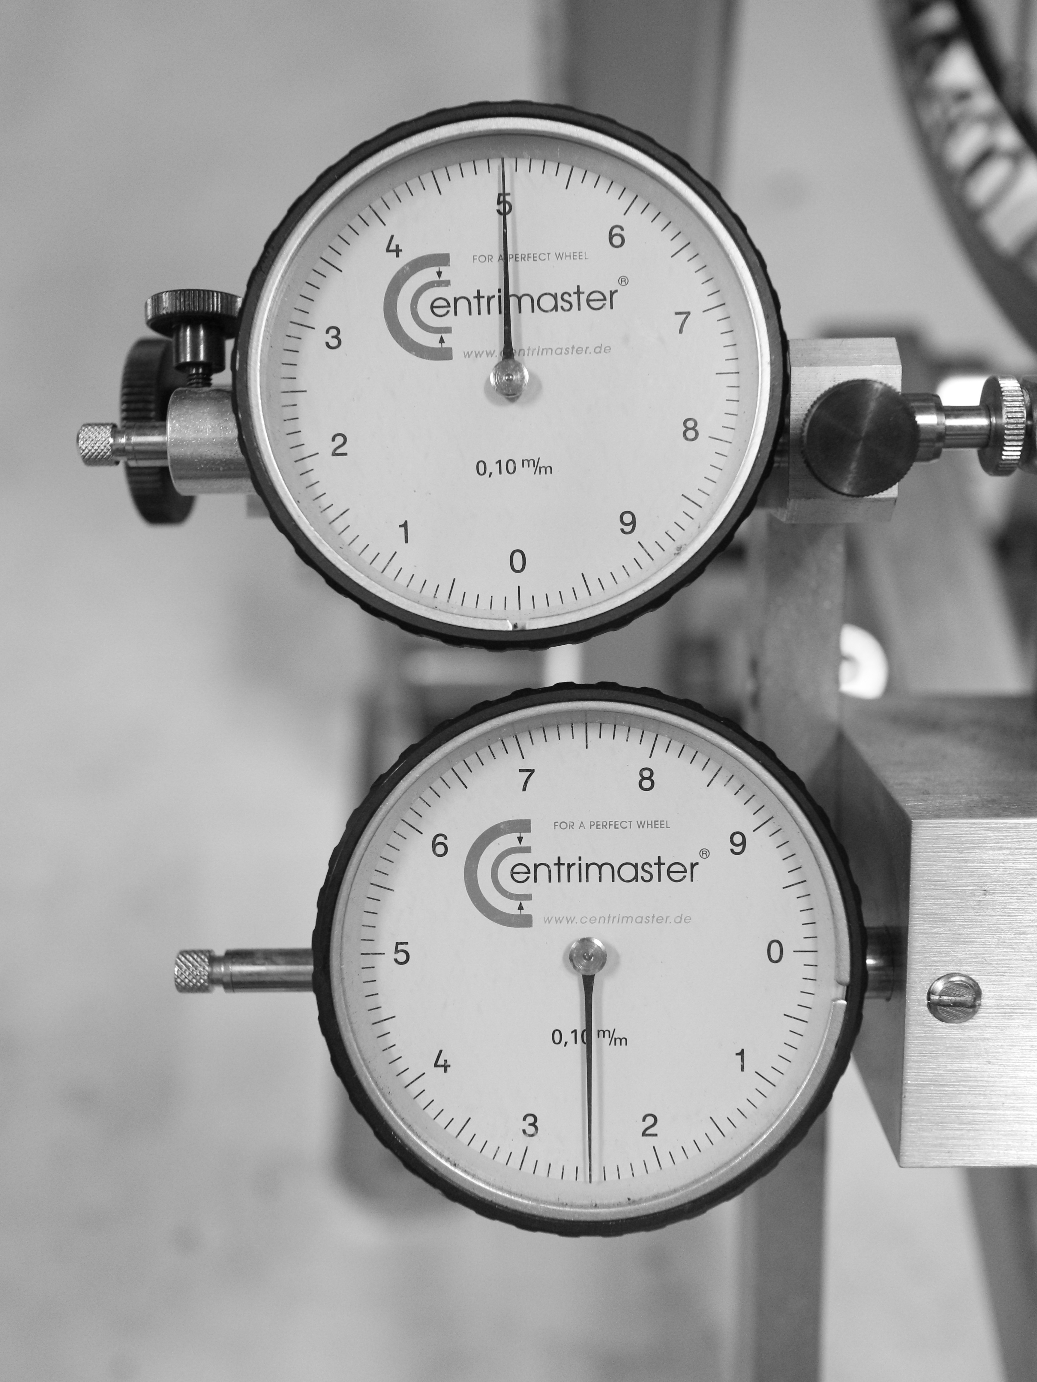
\includegraphics [width = 0.22 \linewidth] {ref.png} 
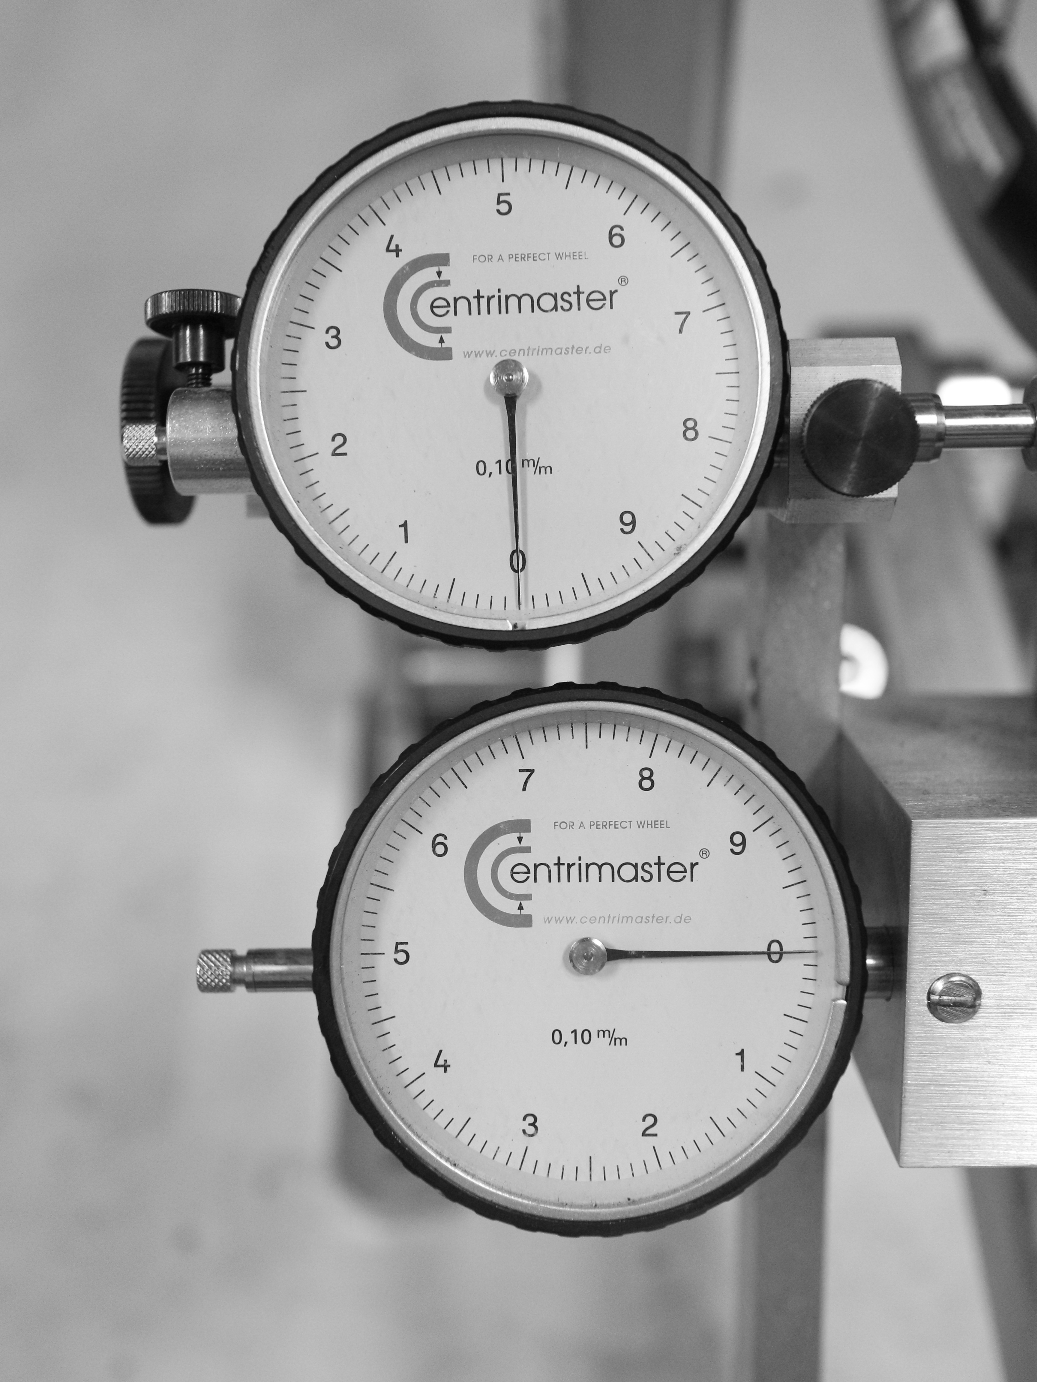
\includegraphics [width = 0.22 \linewidth] {zero.png} 
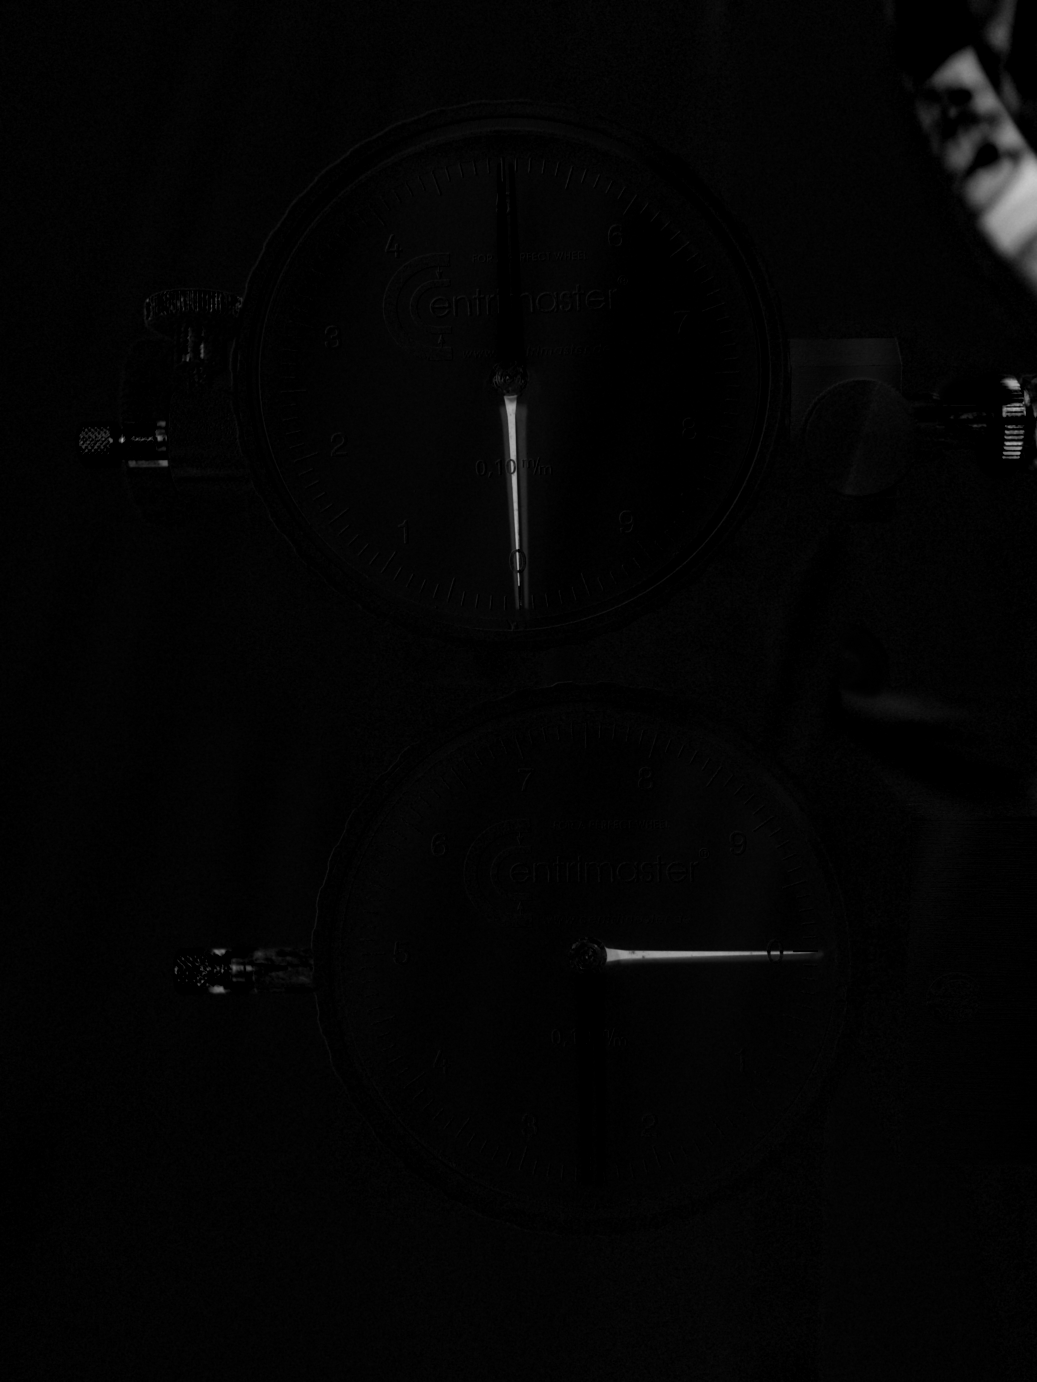
\includegraphics [width = 0.22\linewidth] {delta_img.png} 
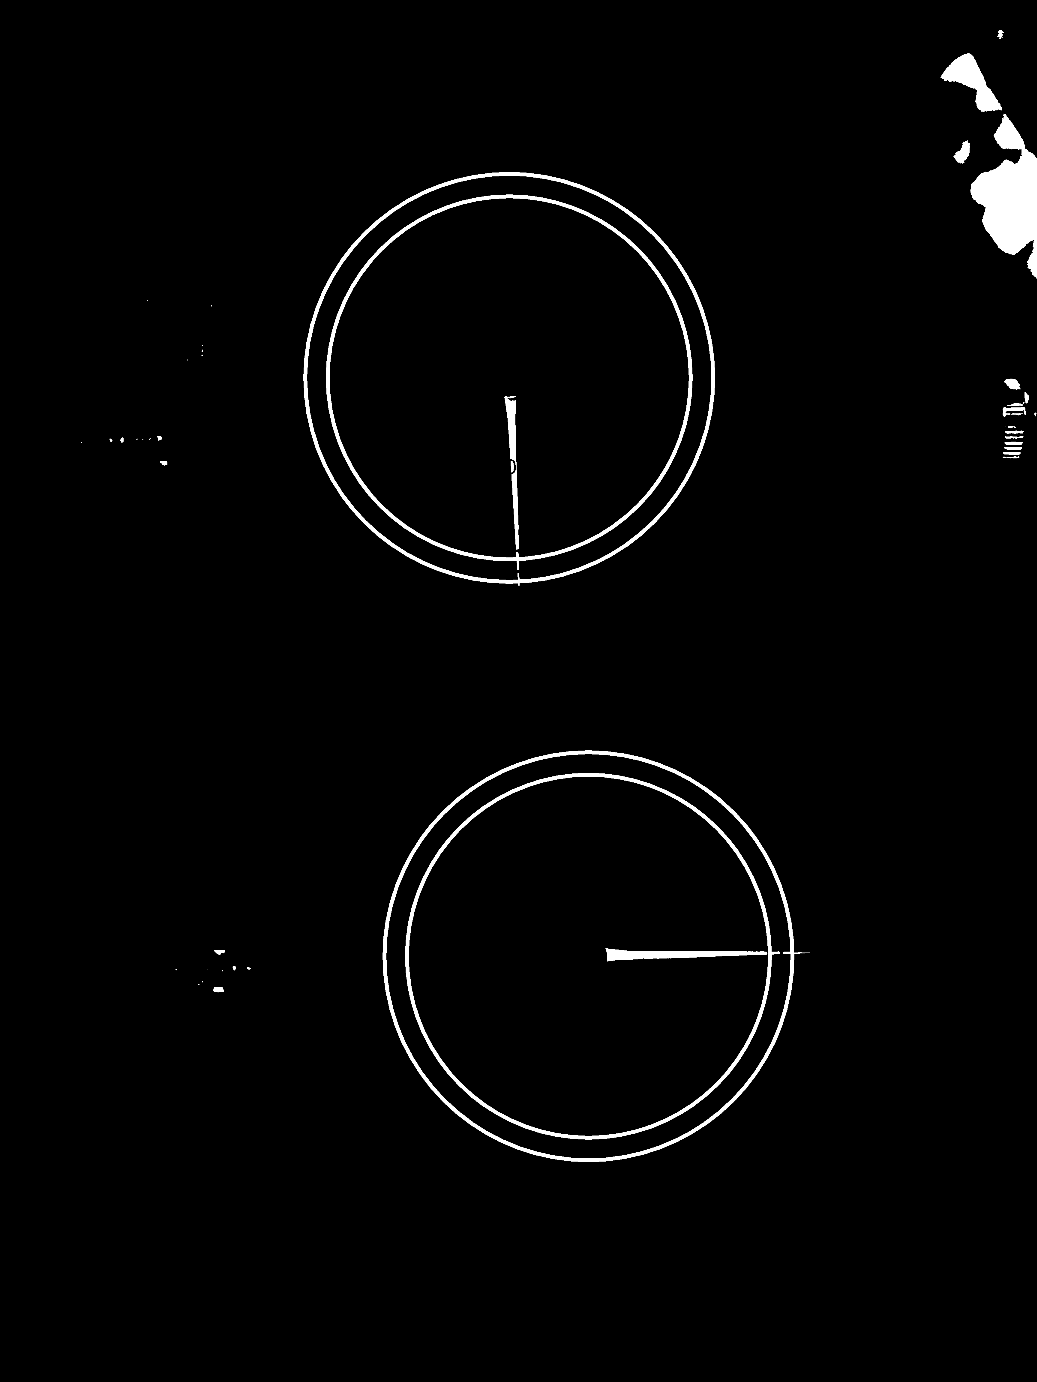
\includegraphics [width = 0.22\linewidth] {threshold_img.png} 
\caption{From left to right: (a) reference image with needles set away from working measurement range.  (b) needles set to zero. (c) second image subtracted from reference image. (d) binary threshold and masking operation, the area masked is between the two circles}
\label{fig:1}
\end{figure}
\FloatBarrier

\end{document}